% --------------------------------------------------------------
% This is all preamble stuff that you don't have to worry about.
% Head down to where it says "Start here"
% --------------------------------------------------------------
 
\documentclass[12pt]{article}
 
\usepackage[margin=1in]{geometry} 
\usepackage{amsmath,amsthm,amssymb}
\usepackage{listings}
\usepackage{bm}
\usepackage{hyperref}
\usepackage{graphicx}
\usepackage{caption}
\usepackage{subfigure}
\usepackage{float}
% \usepackage{subcaption}
\newcommand{\N}{\mathbb{N}}
\newcommand{\Z}{\mathbb{Z}}
 
\newenvironment{theorem}[2][Theorem]{\begin{trivlist}
\item[\hskip \labelsep {\bfseries #1}\hskip \labelsep {\bfseries #2.}]}{\end{trivlist}}
\newenvironment{lemma}[2][Lemma]{\begin{trivlist}
\item[\hskip \labelsep {\bfseries #1}\hskip \labelsep {\bfseries #2.}]}{\end{trivlist}}
\newenvironment{exercise}[2][Exercise]{\begin{trivlist}
\item[\hskip \labelsep {\bfseries #1}\hskip \labelsep {\bfseries #2.}]}{\end{trivlist}}
\newenvironment{reflection}[2][Reflection]{\begin{trivlist}
\item[\hskip \labelsep {\bfseries #1}\hskip \labelsep {\bfseries #2.}]}{\end{trivlist}}
\newenvironment{proposition}[2][Proposition]{\begin{trivlist}
\item[\hskip \labelsep {\bfseries #1}\hskip \labelsep {\bfseries #2.}]}{\end{trivlist}}
\newenvironment{corollary}[2][Corollary]{\begin{trivlist}
\item[\hskip \labelsep {\bfseries #1}\hskip \labelsep {\bfseries #2.}]}{\end{trivlist}}
 
\begin{document}
 
% --------------------------------------------------------------
%                         Start here
% --------------------------------------------------------------
 
%\renewcommand{\qedsymbol}{\filledbox}
 
\title{TalkingData AdTracking Fraud Detection Challenge}%replace X with the appropriate number
\author{Guozhen Li, Hairu Lang \\ %replace with your name
STA 208 - Statistical Machine Learning - Final Project} %if necessary, replace with your course title

\maketitle


\section{Problem Description}
This problem is a data analysis challenge from Kaggle (www.kaggle.com), originally found at  \url{https://www.kaggle.com/c/talkingdata-adtracking-fraud-detection}.
The data provider, TalkingData, tracks a large base of mobile device activity, 
and wants to understand which ad clicks end up with app downloads, 
and which ones lead to nothing (thus are suspects of fraud clicks).
We are provided with a training data set of over 180 million clicks, 
and the objective is to predict whether a click leads to an app download.

For each click, the raw training data set has information about its:
\begin{itemize}
	\item \texttt{ip}: IP address
	\item \texttt{app}: app of marketing
	\item \texttt{device}: device type
	\item \texttt{os}: mobile device operating system type
	\item \texttt{channel}: mobile ad publisher channel
	\item \texttt{click\_time}: click time (date and time, down to seconds)
	\item \texttt{is\_attributed}: whether a download occurs at the end
	\item \texttt{attributed\_time}: download time, if a download occurs
\end{itemize}

This data analysis task poses, at least, the following challenges:
\begin{enumerate}
	\item Extract useful features from the seemingly dispersed information found in the raw training data.
	\item Handling of the extra-large data set (over 180 million samples, as an over 7GB text file), which hardly fits into the memory of a normal personal computer.
	\item Efficient and effective learning method to learn from the data.
\end{enumerate}


\section{Data Exploration}
The training data set has 8 fields, namely ``ip'', ``app'', ``device'', ``os'', ``channel'', ``click\_time'', ``attributed\_time'', and ``is\_attributed''.
Among these, ``ip'' through ``channel'' are categorical features, ``click\_time'' and ``attributed\_time'' are timestamps, and ``is\_attributed'' is the prediction target. 
Fortunately, the data is well-cleaned, and there aren't any missing values except in the ``attributed\_time'' field, which is not surprising because not all clicks led to downloads (i.e. attributed).

We performed some exploratory data analysis in notebook \texttt{python/1 Explore.ipynb}.
The exploration reveals several noticeable facts about the data:
\begin{itemize}
    \item There exist a period of time during a day when clicks and downloads are both low (Figure \ref{fig:activity_by_hour}).
    \item Although the minute-of-hour and second-of-minute of a click doesn't appear significantly correlated to download activities, (click\_minute mod 15) and (click\_second mod 5) seems to seems to do. This might have to do with click-bots that are programmed to ``click'' ads at intervals.
    \item Although there are a huge number of unique IPs, apps, devices, etc. appearing in the training data set, a much smaller number of them show up repeatedly (Figure \ref{fig:unique_values_with_more_activity}). The frequently recurring ones are perhaps targets we want to pay more attention to.
    \item The target feature (whether a click leads to download) in the training data set is highly imbalanced. Only about 0.2\% clicks lead to downloads.
\end{itemize}

\begin{figure}[H]
    \centering
    \subfigure{
        \begin{minipage}{0.45\textwidth}
            \centering
            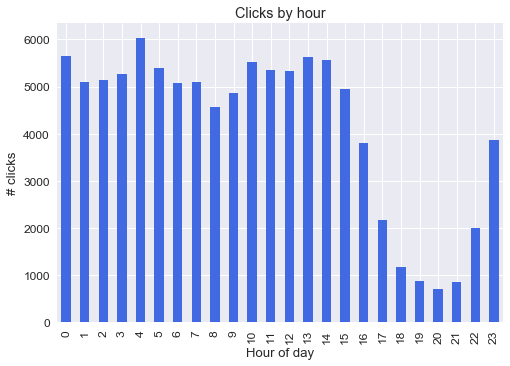
\includegraphics[width=\textwidth]{img/clicks_by_hour.png}
        \end{minipage}
    }
    \subfigure{
        \begin{minipage}{0.45\textwidth}
            \centering
            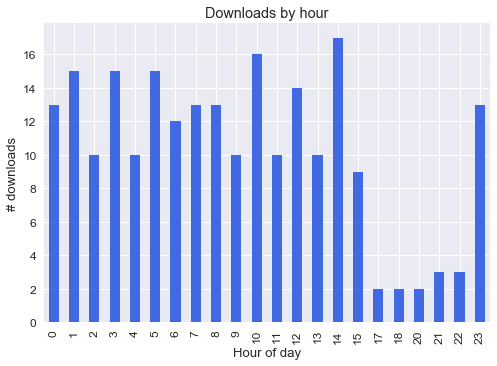
\includegraphics[width=\textwidth]{img/downloads_by_hour.png}
        \end{minipage}
    }
    \caption{User activity by hour of day}
    \label{fig:activity_by_hour}
\end{figure}

\begin{figure}[H]
    \centering
    \subfigure{
        \begin{minipage}{0.45\textwidth}
            \centering
            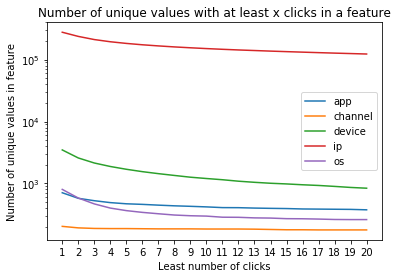
\includegraphics[width=\textwidth]{img/unique_values_with_x_clicks.png}
        \end{minipage}
    }
    \subfigure{
        \begin{minipage}{0.45\textwidth}
            \centering
            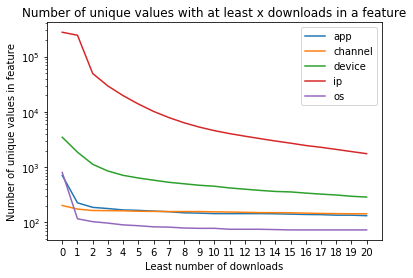
\includegraphics[width=\textwidth]{img/unique_values_with_x_downloads.png}
        \end{minipage}
    }
    \caption{Number of unique values in a feature when filtered for more activities}\label{fig:unique_values_with_more_activity}
\end{figure}


\section{Feature Engineering and Data Pre-processing}
The feature engineering  and data preprocessing work is demonstrated in notebook \texttt{python/2 Feature Engineering and Preprocessing.ipynb}. 
For convenience in later modeling, we also implemented the procedures as a \texttt{Preprocessor} class in \texttt{python/preprocess.py}, 
which can be instantiated and repeatedly used to preprocess a chunk of the training data.

The key actions we took on data preprocessing include:
\begin{itemize}
    \item Extract hour of day, minute of hour, and second of minute from \texttt{click\_time}
    \item Make \texttt{minute\_mod\_15} and \texttt{second\_mod\_5}
    \item Find number of clicks, number of downloads, and downloads-per-click ratio for each IP, each OS, each device, deach app, and each channel, and match these stats to their respective records in training data
    \item One-hot encode IPs, apps, devices, OSes, and chennels that are recurring in the full training data set. Here ``recurring'' is defined as those who made more than 1 download.
\end{itemize}

We also propose two approaches to deal with the large size of the training data: 1) Randomly select a smaller sample for training, or 2) Feed data in small batches and train the model incrementally (a.k.a. online learning).

\section{Modeling and Predicting}

\subsection{Support Vector Machine with RBF Kernel}
We first apply Support Vector Classifier with RBF kernel and tune the parameter for gammas. The relationship between gammas and the accuracy is given by:
\begin{figure}[H]
    \centering
    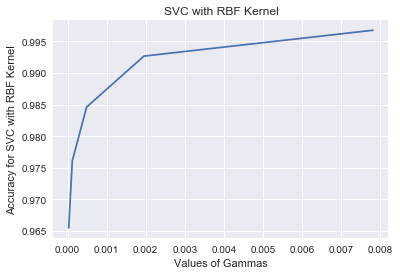
\includegraphics[width=8cm]{img/SVC_RBF/RBF_SVM.png}
\end{figure}
We observe that as gammas increase, the accuracy of prediction is getting larger. The accuracy is high. 

% \subsection{Gradient Tree Boosting with XGBoost}

\subsection{AdaBoostClassifier}
AdaBoostClassifier is a ensemble classifier that combines weaker classifier algorithm to form strong classifier. It generates the optimal classifier by retraining the algorithm iteratively choosing the training set based on accuracy of previous training. We tune two parameter: one is the number of estimators and the other is the maximum depth of the tree. We plot graphs for the relationship between accuracy and the number of estimators, conditional on the maximum depth of the tree. As we change the max depth of the tree (i.e., Decision Tree), the effect of the number of estimators on the accuracy can change a lot. A further inspection reveals that when the depth is one, the accuracy is close to zero. A higher depth can generate accuracies close to 1. Another observation is that the average accuracy corresponding to each max depth gets the highest when the depth is four. Thus, we pick up MaxDepth = 4. Then, we choose 50 to be the number of estimators in our model. The highest accuracy is about 0.99985.
\begin{figure}[H]
    \centering
    \subfigure[MaxDepth=1]{
        \begin{minipage}{4.5cm}
            \centering
            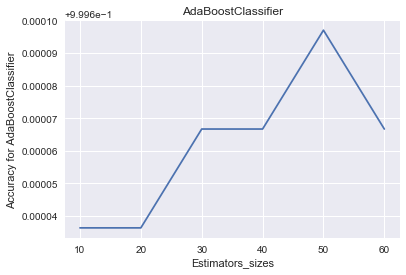
\includegraphics[width=4.5cm]{img/AdaBoostClassifier/Ada_1.png}
        \end{minipage}
    }
    \subfigure[MaxDepth=2]{
        \begin{minipage}{4.5cm}
            \centering
            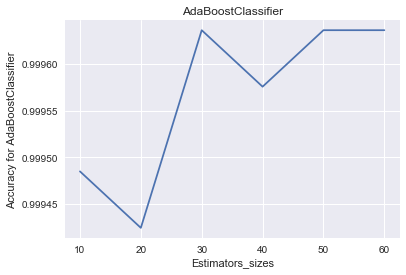
\includegraphics[width=4.5cm]{img/AdaBoostClassifier/Ada_max_2.png}
        \end{minipage}
    }
    \subfigure[MaxDepth=3]{
        \begin{minipage}{4.5cm}
            \centering
            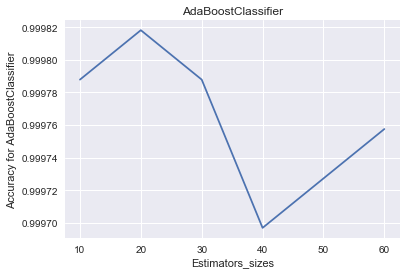
\includegraphics[width=4.5cm]{img/AdaBoostClassifier/Ada_10_max_len_3.png}
        \end{minipage}
    }
\end{figure}

\begin{figure}[H]
    \centering
    \subfigure[MaxDepth=4]{
        \begin{minipage}{4.5cm}
            \centering
            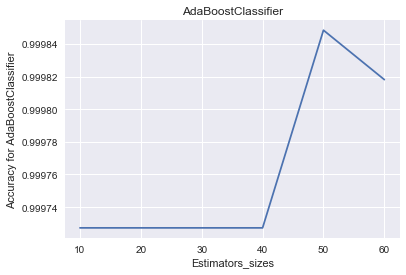
\includegraphics[width=4.5cm]{img/AdaBoostClassifier/Ada_4.png}
        \end{minipage}
    }
    \subfigure[MaxDepth=5]{
        \begin{minipage}{4.5cm}
            \centering
            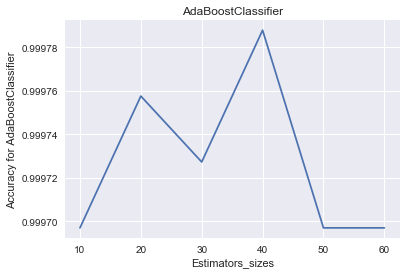
\includegraphics[width=4.5cm]{img/AdaBoostClassifier/Ada_5.png}
        \end{minipage}
    }
    \subfigure[MaxDepth=6]{
        \begin{minipage}{4.5cm}
            \centering
            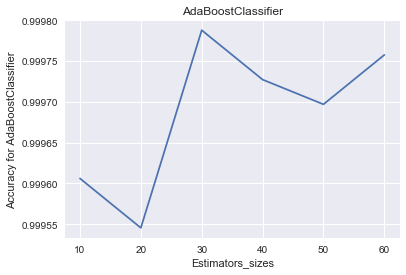
\includegraphics[width=4.5cm]{img/AdaBoostClassifier/Ada_6.png}
        \end{minipage}
    }
\end{figure}


\subsection{Random Forest}
We also implement Random Forest Classification method and tune the parameter for the number of features to consider when looking for the best split, conditional on the number of trees in the forest. The range for the number of estimators is [10, 60] and the range for the maximum number of features is [1, 20]. The following graphs reflect how the maximum number of features influences the prediction accuracy, conditional on the number of estimators.
\begin{figure}[H]
\centering
\subfigure[Random10]{
\begin{minipage}{4.5cm}
\centering
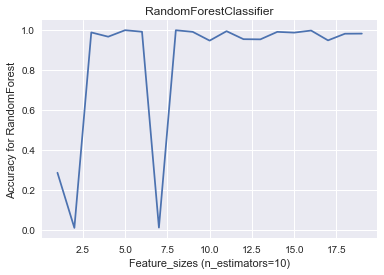
\includegraphics[width=4.5cm]{img/RandomForest/RandomForest10.png}
\end{minipage}
}
\subfigure[Random20]{
\begin{minipage}{4.5cm}
\centering
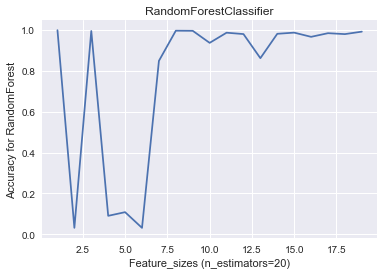
\includegraphics[width=4.5cm]{img/RandomForest/RandomForest20.png}
\end{minipage}
}
\subfigure[Random30]{
\begin{minipage}{4.5cm}
\centering
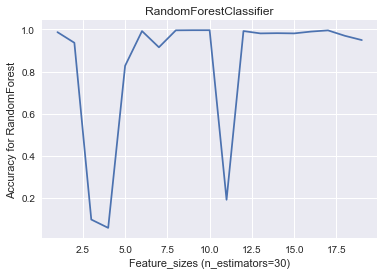
\includegraphics[width=4.5cm]{img/RandomForest/RandomForest30.png}
\end{minipage}
}
\end{figure}

\begin{figure}[H]
\centering
\subfigure[Random40]{
\begin{minipage}{4.5cm}
\centering
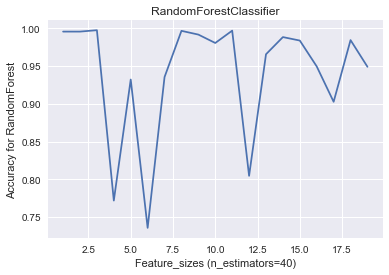
\includegraphics[width=4.5cm]{img/RandomForest/RandomForest40.png}
\end{minipage}
}
\subfigure[Random50]{
\begin{minipage}{4.5cm}
\centering
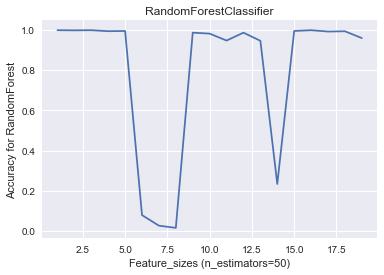
\includegraphics[width=4.5cm]{img/RandomForest/RandomForest1.png}
\end{minipage}
}
\subfigure[Random60]{
\begin{minipage}{4.5cm}
\centering
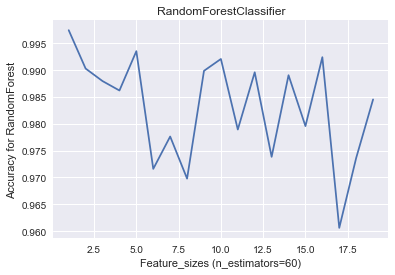
\includegraphics[width=4.5cm]{img/RandomForest/RandomForest60.png}
\end{minipage}
}
\end{figure}
Based on above results, we can see that as we increase the number of estimators, the accuracy of prediction is decreasing, contrary to the theory. The possible reason is that an accurate forest consists of diverse and accurate models. When the size of the forest is getting larger, it  becomes more difficult to generate a new diverse model. Thus, adding one tree which is not diverse enough would not lead to the improvement of the performance. We would choose 10 for the number of estimators. Based on the first graph, when the number of features is 5, 8, 12, the precision is close to one.  

\subsection{LightGBM}
LightGBM is a gradient boosting framework that uses tree-based on learning algorithm. It is relatively new but powerful. Compared with other tree-based algorithms, it grows tree vertically. The main advantanges of LightGBM are that it can handle large size of data, taking lower memory to run and focuses on accuracy of results. We implement LightGBM algorithm to make prediction and tune the values of parameter learning rate, conditional on the number of leaves. The relationships between the accuracy and learning rates are given by:
\begin{figure}[H]
\centering
\subfigure[NumLeaves20]{
\begin{minipage}{4.5cm}
\centering
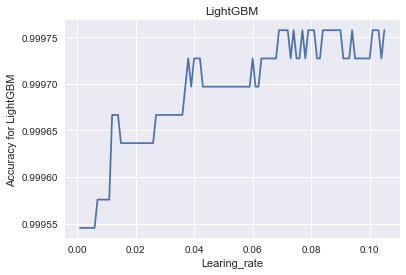
\includegraphics[width=4.5cm]{img/LightGBM/Light_Num_20.png}
\end{minipage}
}
\subfigure[NumLeaves25]{
\begin{minipage}{4.5cm}
\centering
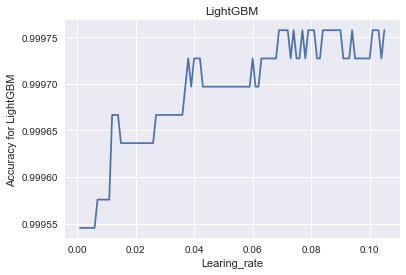
\includegraphics[width=4.5cm]{img/LightGBM/Light_Num_25.png}
\end{minipage}
}
\subfigure[NumLeaves30]{
\begin{minipage}{4.5cm}
\centering
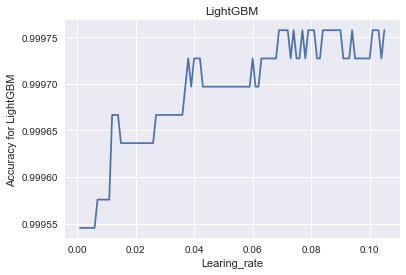
\includegraphics[width=4.5cm]{img/LightGBM/Light_Num_30.png}
\end{minipage}
}
\end{figure}

\begin{figure}[H]
\centering
\subfigure[NumLeaves35]{
\begin{minipage}{4.5cm}
\centering
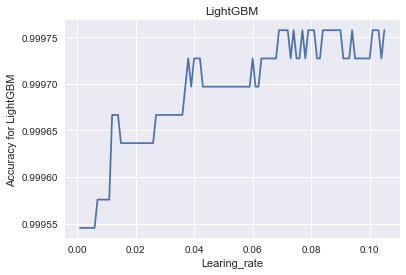
\includegraphics[width=4.5cm]{img/LightGBM/Light_Num_35.png}
\end{minipage}
}
\subfigure[NumLeaves40]{
\begin{minipage}{4.5cm}
\centering
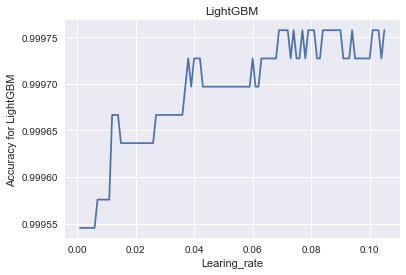
\includegraphics[width=4.5cm]{img/LightGBM/Light_Num_40.png}
\end{minipage}
}
\subfigure[NumLeaves45]{
\begin{minipage}{4.5cm}
\centering
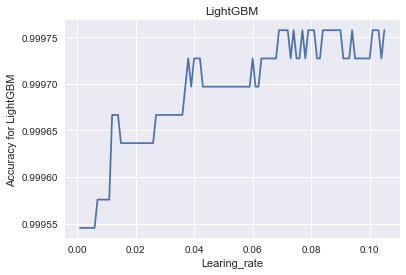
\includegraphics[width=4.5cm]{img/LightGBM/Light_Num_45.png}
\end{minipage}
}
\end{figure}
Based on above graphs, the number of leaves does not make big differences. As we tune the number of leaves, the relationship between the accuracy of prediction and learning rates does not change much. The consistent result from those graphs is that as we increase the learning rate to 0.11, the accuracy is higher. We set the value of the number of leaves to be 30 and choose 0.102 as the learning rate. The highest accuracy is also higher than 0.99975.

\section{Model Evaluation and Conclusions}
First, both AdaBoostClassifier and LightGBM can generate high accuracies of prediction. Random Forest classifier and SVM with RBF Kernel, however, can generate relatively low accuraries sometimes. Second, the prediction results from AdaBoostClassifier and Random Forest classifier can be sensitive to the changes in the parameters and the way to split the data. Prediction from LightGBM is not sensitive to the parameter changes or respond to the changes in a matter that can be expected. As for the running time, the implementation of AdaBoostClassifier and SVC with RBF Kernel can be quite time-consuming; however, the implementation of LightGBM can take much shorter time. Overall, we will choose LightGBM as our prediction model and choose the learning rate as 0.1.
 
% --------------------------------------------------------------
%     You don't have to mess with anything below this line.
% --------------------------------------------------------------
 
\end{document}